%%%%%%%%%%%%%%%%%%%%%%%%%%%%%%%%%%%%%%%%%%%%%%%%%%%%%%%%%%%%%%%%%%%%%%%%%%%%%%%
\section{Validating the OpenMC MGXS Generation Module}
\label{sec:validate}
%%%%%%%%%%%%%%%%%%%%%%%%%%%%%%%%%%%%%%%%%%%%%%%%%%%%%%%%%%%%%%%%%%%%%%%%%%%%%%%

This section provides a case study to validate the \texttt{openmc.mgxs} module. \cref{subsec:benchmarks} introduces two pressurized water reactor (PWR) benchmarks, and the reference results computed with OpenMC. MGXS were generated with \texttt{openmc.mgxs} for both benchmarks as discussed in \cref{subsec:openmc} and then used for multigroup calculations with the OpenMOC code highlighted in \cref{subsec:openmoc}. The continuous-energy and multigroup solutions are compared in \cref{subsec:results}.


%%%%%%%%%%%%%%%%%%%%%%%%%%%%%%%%%%%%%%%%%%%%%
\subsection{Benchmarks and Reference Results}
\label{subsec:benchmarks}

Two benchmarks were derived from the Benchmark for Evaluation And Validation of Reactor Simulations (BEAVRS) PWR model~\cite{horelik2013beavrs} to validate the \texttt{openmc.mgxs} module. Both benchmarks included a heterogeneous composition of 1.6\% and 3.1\% enriched UO$_2$ fuel, borated water, zircaloy, helium, air, borosilicate glass and stainless steel. The isotopic compositions of the materials and the geometric configurations of each pin type were identical to those given in the BEAVRS specifications and are not reproduced here. The continuous energy cross sections were from the ENDF/B-VII.1 library~\cite{mcnpx2003manual} evaluated at 600K for hot power conditions.

The two benchmarks are illustrated in \cref{fig:benchmarks-materials}. The first benchmark was a fuel assembly comprising 264 pins of 1.6\% enriched fuel, 24 control rod guide tubes (CRGTs), and a single central instrument tube. The assembly was modeled with reflective boundary conditions. The second benchmark was a 2$\times$2 colorset of fuel assemblies surrounded by a water reflector on the bottom and right. The top-left and bottom-right fuel assemblies were identical to the single assembly benchmark. The top-right and bottom-left assemblies comprised 264 pins of 3.1\% enriched fuel, 20 CRGTs, four burnable poisons (BPs), and a central instrument tube. The colorset was modeled with reflective boundaries on the top and left and vacuum boundaries on the bottom and right. Although BEAVRS is an axially heterogeneous 3D core model, both benchmarks were fabricated in 2D because of the geometric constraints in OpenMOC.

\begin{figure}[h!]
\centering
\begin{subfigure}{0.45\textwidth}
  \centering
  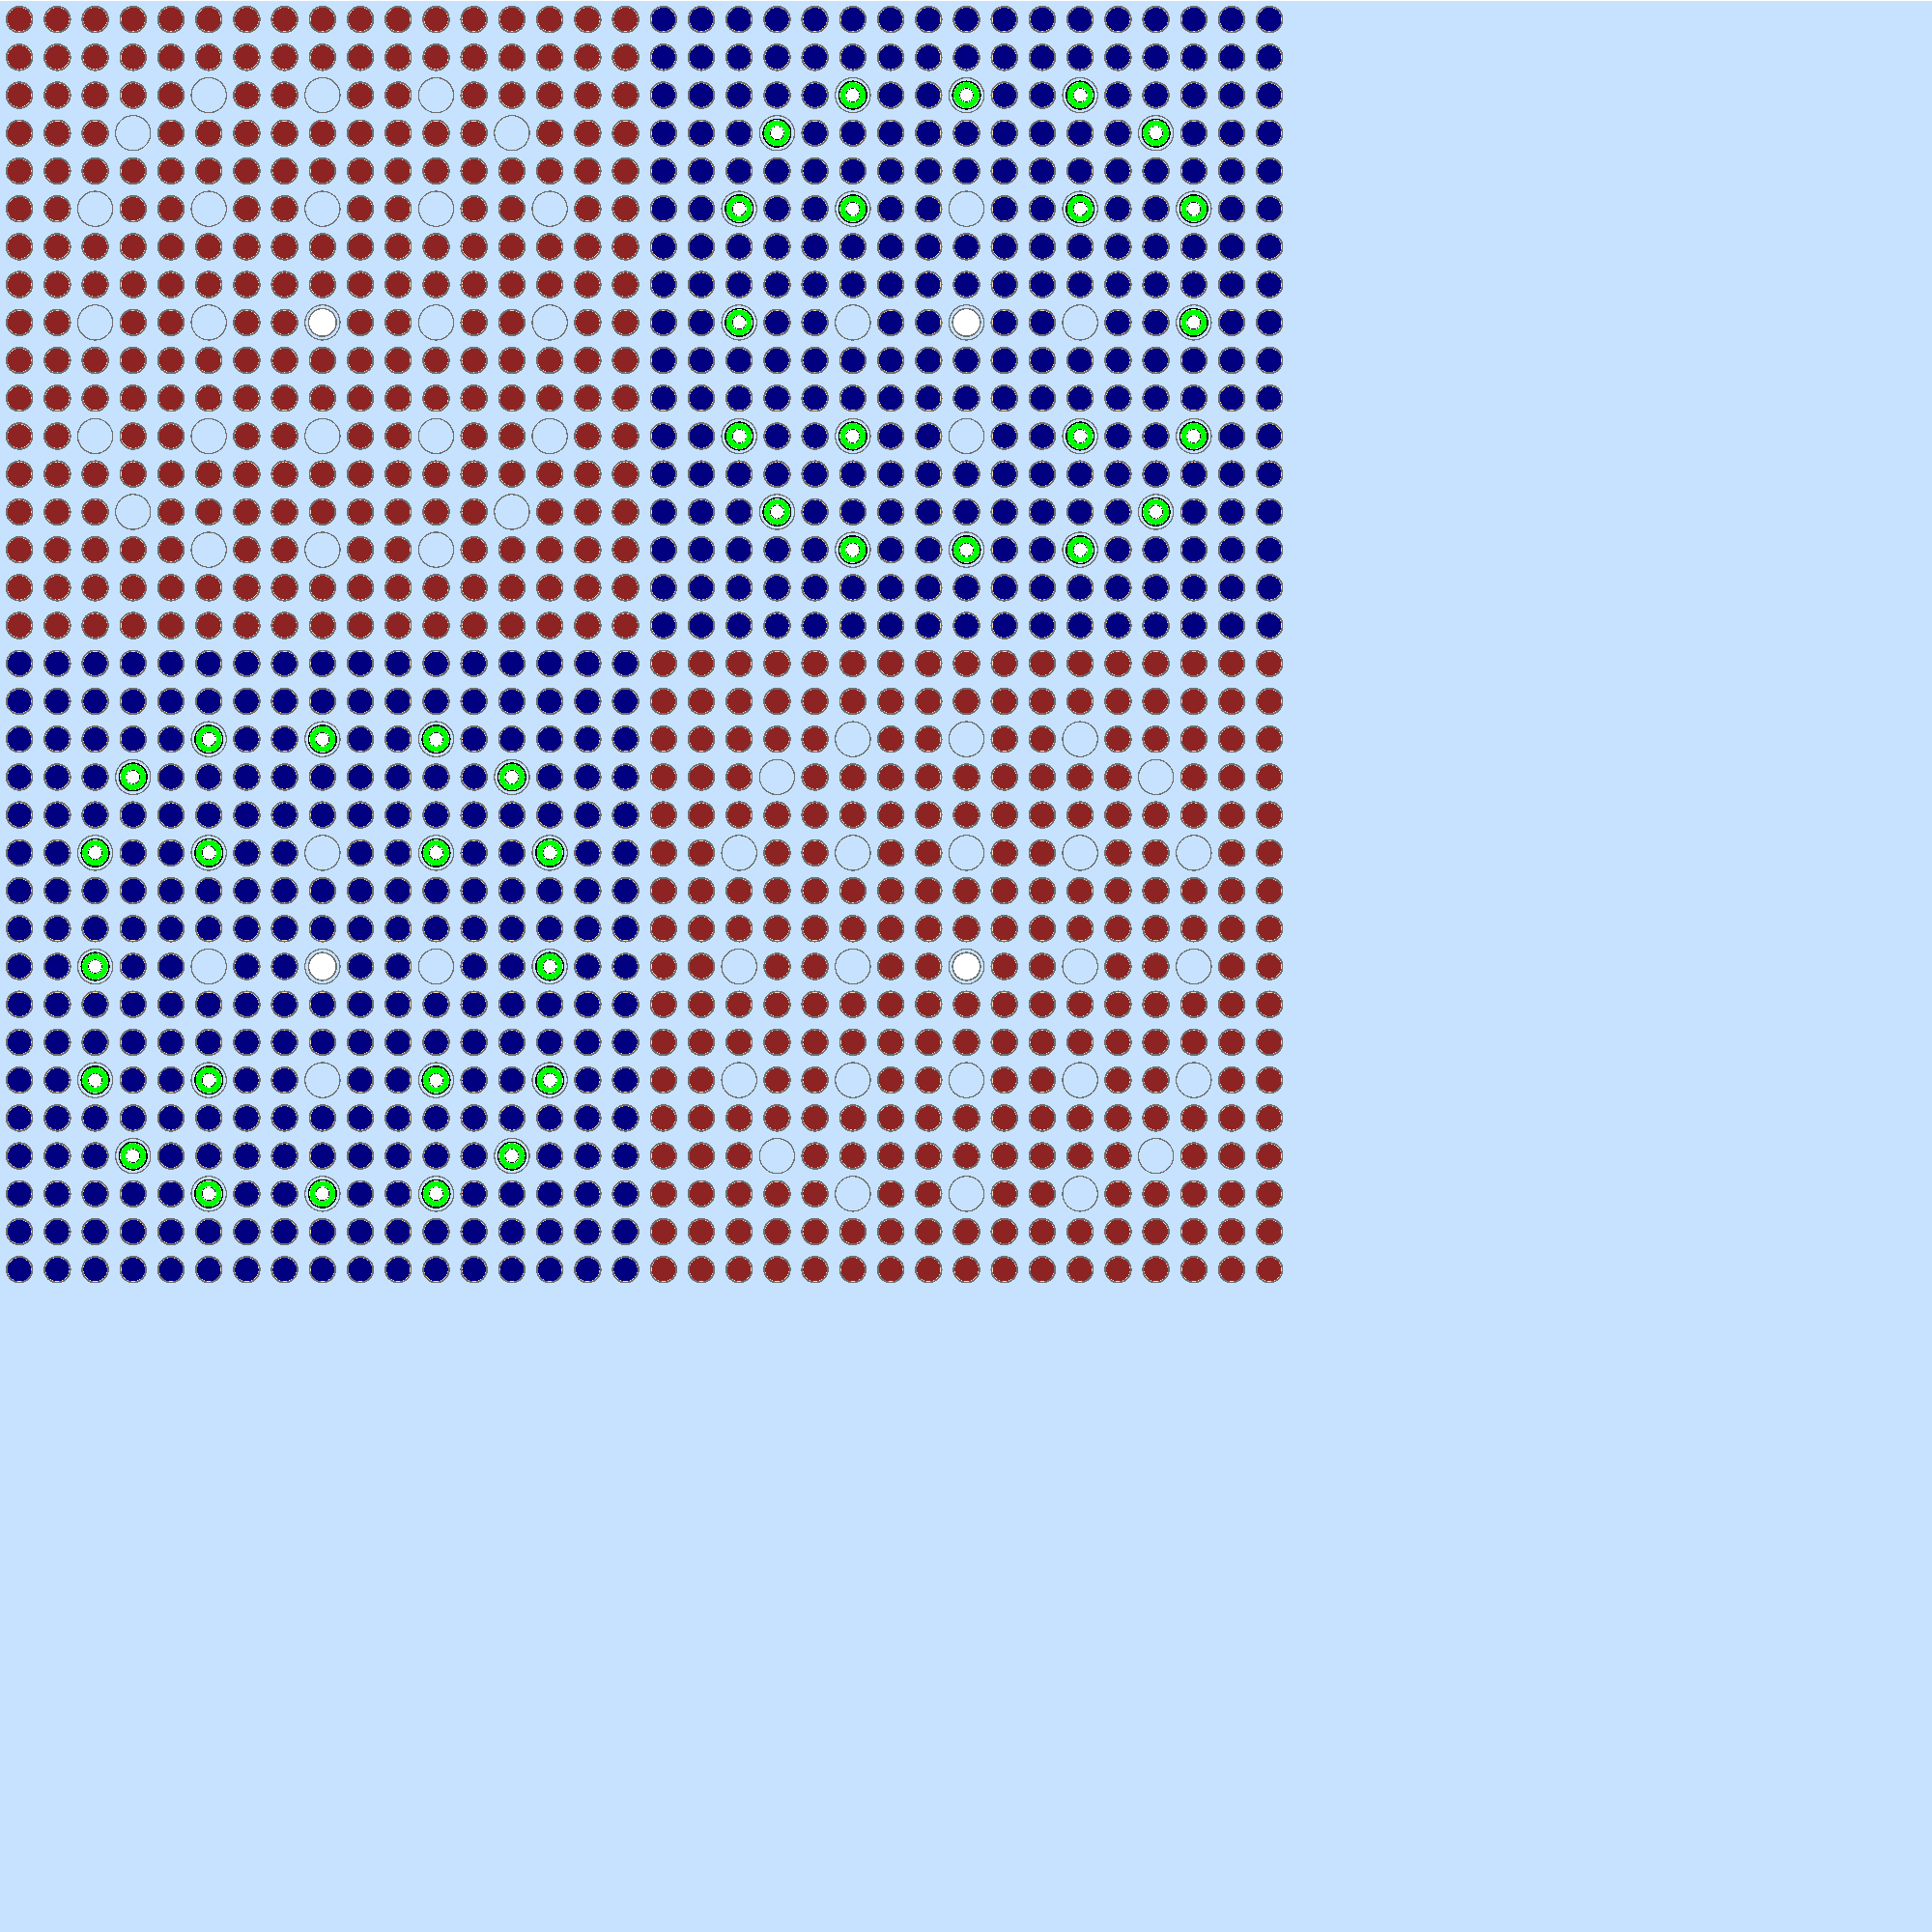
\includegraphics[width=0.8\linewidth]{figures/assm_geometry}
  \caption{}
  \label{fig:benchmarks}
\end{subfigure}
\begin{subfigure}{0.45\textwidth}
  \centering
  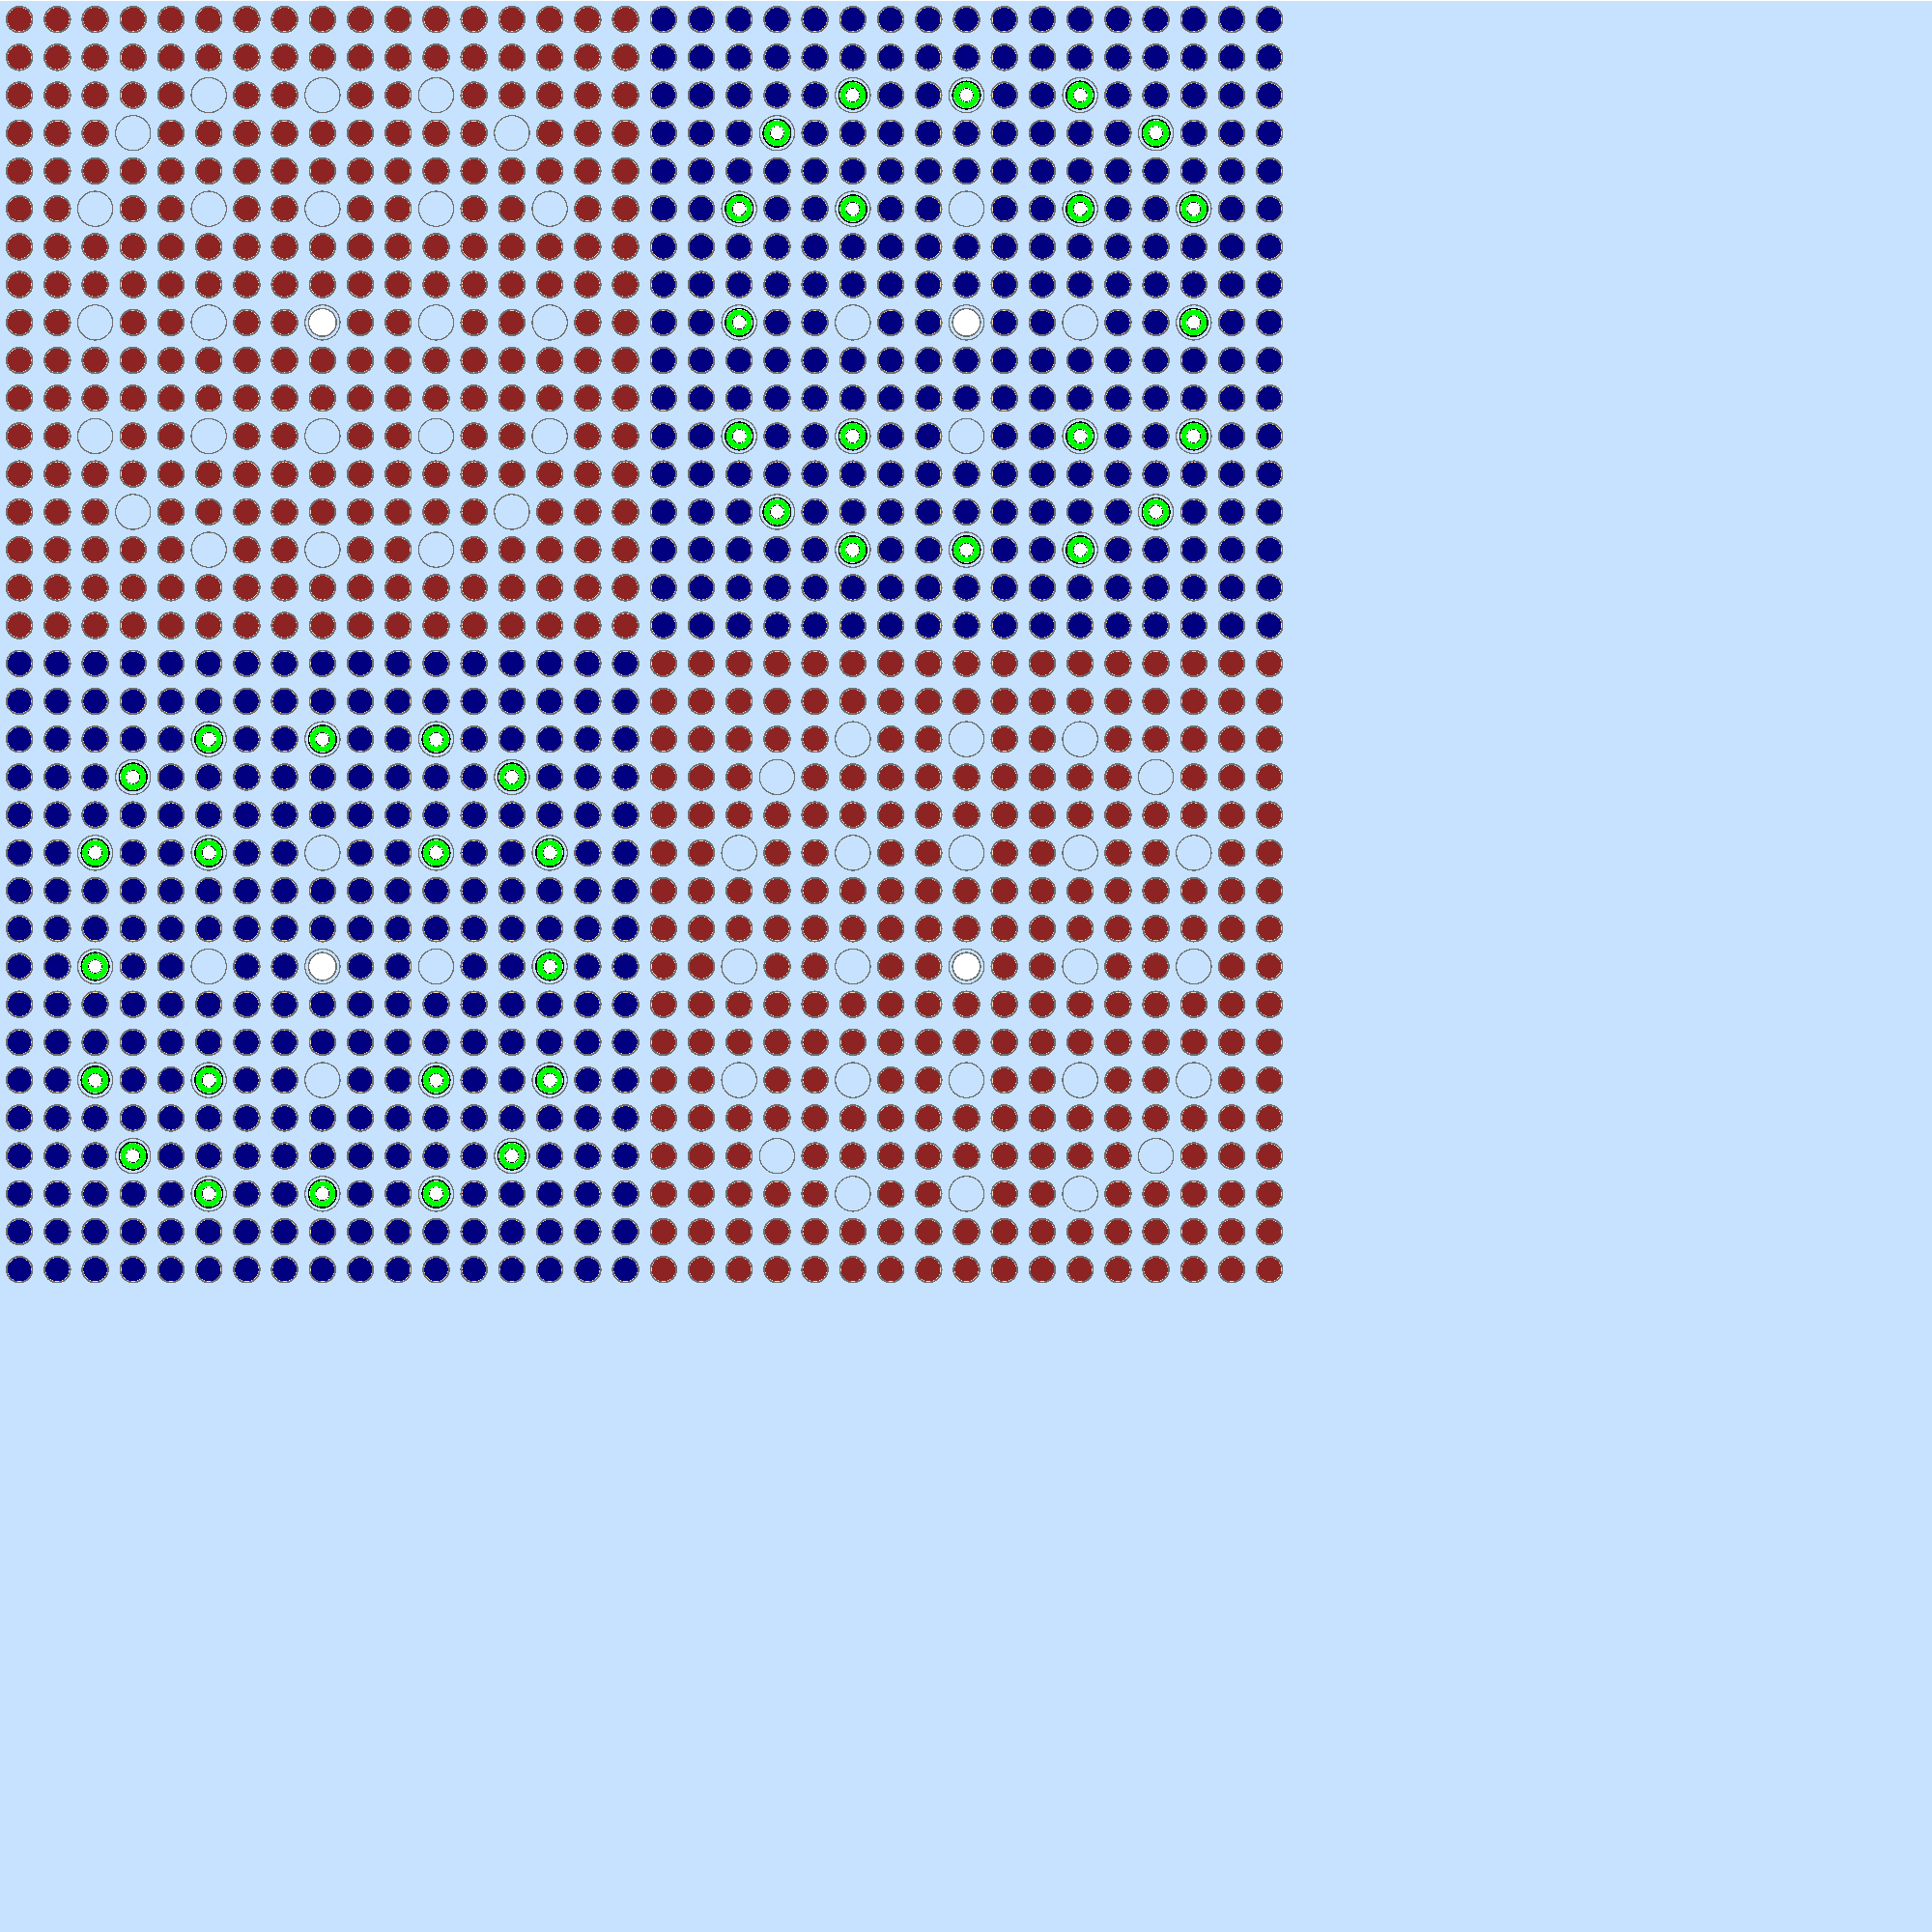
\includegraphics[width=0.8\linewidth]{figures/colorset_geometry}
  \caption{}
  \label{fig:benchmarks-colorset}
\end{subfigure}
\caption{Assembly (a) and colorset (b) benchmark geometries.}
\label{fig:benchmarks-materials}
\end{figure}

OpenMC simulations were used to compute both the MGXS and reference eigenvalues and pin-wise fission rates for both benchmarks. The reference solutions were computed with 100 inactive and 900 active batches of 10$^7$ particles histories per batch. The OpenMC reference eigenvalues and their associated 1-sigma uncertainties are reported in \cref{tab:keff-reference}. Rectilinear, pin-wise tally meshes were used to compute the reference energy-integrated fission rate spatial distributions shown in \cref{fig:benchmarks-fiss-rates}. The fission rates were normalized to the mean of the nonzero fission rates. The rates in the CRGTs, BPs, and instrument tubes are all zero and are shaded in white. The fission rates have 1-sigma uncertainties of less than 0.08\%.

\begin{table}[h!]
  \centering
  \caption{Reference OpenMC eigenvalues for each benchmark.}
  \label{tab:keff-reference}
  \begin{tabular}{c c}
  \toprule
  {\bf Assembly} &
  {\bf Colorset} \\
  \midrule
  0.99326 $\pm$ 0.00001 & 0.94574 $\pm$ 0.00001 \\
  \bottomrule
\end{tabular}
\end{table}

\begin{figure*}[h!]
\centering
\begin{subfigure}{0.45\textwidth}
  \centering
  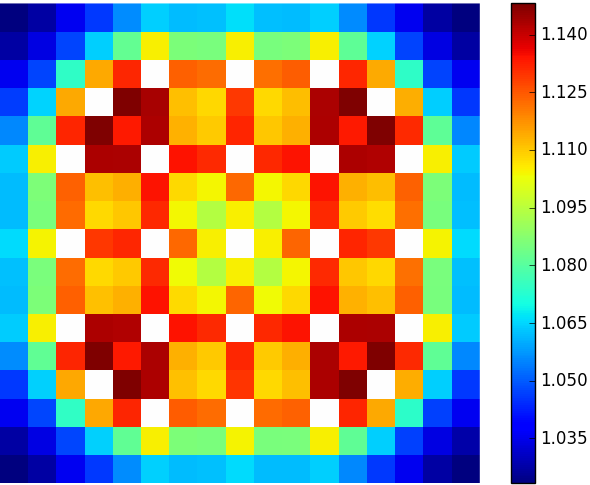
\includegraphics[width=0.8\linewidth]{figures/assm_fiss_rates}
  \caption{}
  \label{fig:fiss-assm}
\end{subfigure}%
\begin{subfigure}{0.45\textwidth}
  \centering
  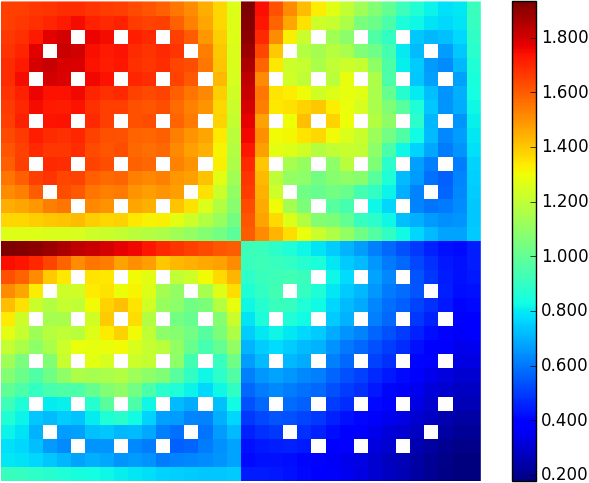
\includegraphics[width=0.8\linewidth]{figures/colorset_fiss_rates}
  \caption{}
  \label{fig:capt-assm}
\end{subfigure}
\caption{Normalized reference OpenMC fission rates for the assembly (a) and colorset (b) benchmarks.}
\label{fig:benchmarks-fiss-rates}
\end{figure*}


%%%%%%%%%%%%%%%%%%%%%%%%%%%%%%%%%%%%%%%%%%%%%%%%%%%%%%%%%%%%
\subsection{MGXS Generation with OpenMC}
\label{subsec:openmc}

The \texttt{openmc.mgxs} module was employed to generate MGXS tallied in CASMO's 70 energy group structure \cite{rhodes2006casmo}. Two OpenMC eigenvalue calculations were performed for the 1.6\% and 3.1\% enriched fuel pins, each in an infinite, repeating array\footnote{An infinite, repeating array of fuel pins is modeled by a single fuel pin with reflective boundary conditions.}, to generate MGXS for the fuel, zircaloy cladding, helium gap, and borated water moderator. An additional OpenMC eigenvalue calculation of the entire geometry for each benchmark was performed to generate MGXS for those pins lacking fissile materials (CRGTs, BPs, instrument tubes and the reflector). The 70-group MGXS were subsequently condensed to CASMO's 8- and 2-group structures by using the \texttt{openmc.mgxs} module's data-processing features. This two-step approach with two MC calculations was used as a proxy for traditional MGXS generation for lattice physics calculations which separately treat fissile and non-fissile pins. Future work may develop a streamlined framework to generate MGXS for all pins simultaneously using a single MC calculation.

Each OpenMC simulation included 100 inactive and 900 active batches of 10$^{6}$ particle histories per batch. The OpenMC simulations used the iso-in-lab feature to eliminate scattering source anisotropy as one possible cause of approximation error between OpenMC and OpenMOC. \textcolor{red}{The iso-in-lab feature eliminates hydrogen anisotropy of the water reflector and the need for a transport correction. It is emphasized that the iso-in-lab approximation is quite limiting in its applicability for real-world use cases, such as burn-up calculations for light water reactors. Nevertheless, the approximation was employed to demonstrate the efficacy of OpenMC's MGXS generation module since OpenMOC's current implementation is limited to using an isotropic scattering source. Although transport-corrected cross sections could be used rather than the iso-in-lab approximation, they would have made it more challenging to isolate, examine, and understand the approximation error between OpenMC and OpenMOC.}

%%%%%%%%%%%%%%%%%%%%%%%%%%%%%%%%%%%%%%%%%%%%%%%%%%%%%%%%%%%%
\subsection{Multigroup Calculations with OpenMOC}
\label{subsec:openmoc}

The MGXS generated by OpenMC were supplied to OpenMOC \cite{boyd2014openmoc} for deterministic multigroup transport calculations. The OpenMOC code solves the method of characteristics form of the neutron transport equation for 2D fixed source and eigenvalue calculations. OpenMOC approximates the scattering source as isotropic and the neutron source as constant across each spatial zone. The OpenMOC simulations used a characteristic track laydown with 128 azimuthal angles and 0.05 cm spacing with the Tabuchi-Yamamoto three polar angle (TY3) quadrature set \cite{yamamoto2007}. The UO$_2$ fuel pins and CRGTs were subdivided into five and ten equal volume radial rings, respectively. The burnable poison pins were discretized with five equal volume radial rings in both the borosilicate glass and borated water material zones. The moderator surrounding each pin was subdived with five equally spaced rings. Eight equal angle subdivisions were applied to all material zones. The root mean square of the energy-integrated fission source in each spatial zone was converged to 10$^{-5}$. The eigenvalues and pin-wise fission rates computed by OpenMOC are compared with the OpenMC reference solutions for both benchmarks in the following section.


%%%%%%%%%%%%%%%%%%%%%%%%%%%%%%%%%%%%%%%%%%%%%%%%%%%%%%%%%%%%%%%%%%%%%%%%%%%%%%%
\subsection{Results}
\label{subsec:results}
%%%%%%%%%%%%%%%%%%%%%%%%%%%%%%%%%%%%%%%%%%%%%%%%%%%%%%%%%%%%%%%%%%%%%%%%%%%%%%%

The OpenMOC eigenvalues were compared with the reference OpenMC eigenvalues from \cref{tab:keff-reference}. The eigenvalue bias $\Delta k$ was calculated by comparing the eigenvalue $k_{\textrm{eff}}^{\textrm{MOC}}$ from OpenMOC to the reference eigenvalue $k_{\textrm{eff}}^{\textrm{MC}}$ computed by OpenMC in units of per cent mille (pcm):

\begin{equation}
\label{eqn:delta-rho}
\Delta k = \left(k_{\textrm{eff}}^{\textrm{MOC}} - k_{\textrm{eff}}^{\textrm{MC}}\right) \times 10^{5}
\end{equation}

The bias is listed for both benchmarks in \cref{tab:keff-bias} for 2-, 8-, and 70-group structures. As expected, the eigenvalue bias is highly dependent on the energy group structure and improves as the energy discretization is refined. The 70-group eigenvalues are consistent with OpenMC to within 50 pcm for both benchmarks, demonstrating that global reaction rates are preserved with MGXS generated by OpenMC. It should be noted, however, that quite different biases would be expected if anisotropic scattering were employed in OpenMC without a robust implementation of a higher-order scattering kernel in OpenMOC.

\begin{table}[h!]
  \centering
  \caption{OpenMOC eigenvalue bias $\Delta k$.}
  \label{tab:keff-bias}
  \begin{tabular}{l r r r}
  \toprule
  \textbf{Benchmark} & \textbf{2-Group} & \textbf{8-Group} & \textbf{70-Group} \\
  \midrule
  Assembly & -132 & -68 & 31 \\
  \midrule
  Colorset & 2103 & 267 & 46 \\
  \bottomrule
\end{tabular}
\end{table}

The OpenMOC energy-integrated pin-wise fission rates were compared with the reference OpenMC fission rates in \cref{fig:benchmarks-fiss-rates}. The percent relative errors for each pin's fission rates were computed, and the maximum and mean errors are listed in \cref{tab:fiss-errors}. In particular, the maximum errors are the maximum of the absolute values of the errors along with the appropriate sign, while the mean errors are the averages of the absolute error magnitudes. The spatial distributions of fission rate errors with 70 groups are plotted as heatmaps for both benchmarks in \cref{fig:fiss-errors}. These results demonstrate that pin-wise fission rates can be predicted to within 1\% accuracy with MGXS generated from OpenMC if the energy discretization is sufficiently refined. The systematic trends in the spatial distributions---specifically, the fission rates are generally overpredicted for pins near the reflector and underpredicted for pins along the inter-assembly interfaces of the colorset benchmark---are likely due to the fact that the moderating effects of the nearby reflector and/or CRGTs are not accounted for in the MGXS generated for the fuel pins. Future work may develop techniques to account for these spatial self-shielding effects using the \texttt{openmc.mgxs} module.

\textcolor{red}{These results confirm the expectation that multi-group calculations with finer energy discretizations should in general be more consistent with Monte Carlo reference solutions. However, it is emphasized that while these results illustrate the effectiveness of OpenMC's MGXS generation module, they are not intended to provide comprehensive guidance on the efficacy of different energy group structures for solving high-fidelity neutron transport problems.}

\begin{table}[h!]
  \centering
  \caption{OpenMOC max and mean fission rate percent relative errors.}
  \label{tab:fiss-errors}
  \begin{tabular}{l l r r r}
  \toprule
  \textbf{Benchmark} & \textbf{Metric} & \textbf{2-Group} & \textbf{8-Group} & \textbf{70-Group} \\
  \midrule
  \multirow{2}{*}{Assembly} & Max  & 2.387 & 0.643 & 0.375 \\
                            & Mean & 0.951 & 0.231 & 0.073 \\
  \midrule
  \multirow{2}{*}{Colorset} & Max  & 11.024 & 2.773 & 0.670 \\
                            & Mean & 4.964  & 1.029 & 0.147 \\
  \bottomrule
\end{tabular}
\end{table}

\begin{figure*}[h!]
\centering
\begin{subfigure}{0.45\textwidth}
  \centering
  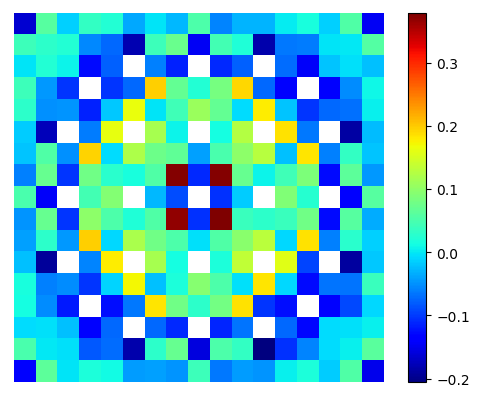
\includegraphics[width=\linewidth]{figures/assm_fiss_errors}
  \caption{}
  \label{fig:assm-fiss-single-step-error}
\end{subfigure}%
\begin{subfigure}{0.45\textwidth}
  \centering
  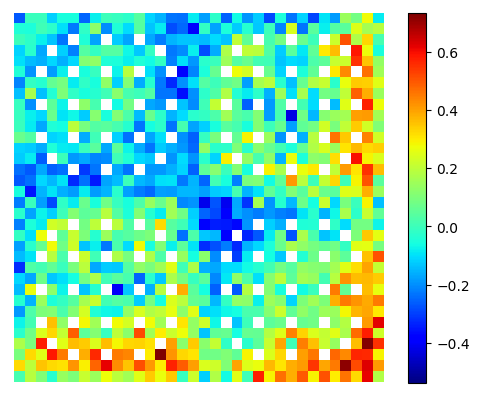
\includegraphics[width=\linewidth]{figures/colorset_fiss_errors}
  \caption{}
  \label{fig:colorset-fiss-single-step-error}
\end{subfigure}
\caption{OpenMOC fission rate percent relative errors for the assembly (a) and colorset (b) benchmarks.}
\label{fig:fiss-errors}
\end{figure*}
